\documentclass[12pt]{article}

\usepackage{sbc-template}

\usepackage{graphicx,url}

\usepackage{algorithm}
\usepackage{algpseudocode}

\usepackage{amssymb}
\usepackage{mathtools}

%\usepackage[brazil]{babel}   
\usepackage[latin1]{inputenc}  
     
\sloppy

\title{UKP5: Solving the Unbounded Knapsack Problem}

\author{Henrique Becker \and Luciana S. Buriol}

\address{Instituto de Inform�tica -- Universidade Federal do Rio Grande do Sul
  (UFRGS)\\
  Caixa Postal 15.064 -- 91.501-970 -- Porto Alegre -- RS -- Brazil
  \email{\{hbecker,buriol\}@inf.ufrgs.br}
}

\begin{document} 

\maketitle

\begin{abstract}
In this extended abstract % resumo extendido -- short paper?
we present UKP5, an algorithm for solving the unbounded knapsack problem. 
UKP5 is based on dynamic programming, but implemented in a non traditional way: instead of looking backward for stored values of subproblems, it stores incremental lower bounds forward. 
%UKP5 uses sparsity, periodicity, and dominance for speeding up computation. 
UKP5 is considerably simpler than EDUK2, the state-of-the-art algorithm for solving the problem. 
%Moreover, it can be naturally implemented using the imperative paradigm, differently from EDUK2. 
We run UKP5 and EDUK2 on a benchmark of 4540 hard instances proposed by the authors of EDUK2. 
The results reveal that UKP5 outperforms EDUK2, being 47 times faster on the average.
\end{abstract}

\begin{resumo}
Nesse resumo extendido n�s apresentamos o UKP5, um algoritmo para solucionar o \emph{unbounded knapsack problem} (problema da mochila com repeti��es).
O UKP5 � baseado em programa��o din�mica, mas implementado de uma forma n�o-tradicional: ao inv�s de olhar para tr�s para usar solu��es de subproblemas previamente computados, ele armazena limites inferiores a frente.
%UKP5 uses sparsity, periodicity, and dominance for speeding up computation. 
O UKP5 � consideravelmente mais simples que o EDUK2, o algoritmo do estado da arte para solucionar o problema.
%Moreover, it can be naturally implemented using the imperative paradigm, differently from EDUK2. 
N�s executamos o UKP5 e o EDUK2 em uma bateria de testes contendo 4540 inst�ncias conside-radas dif�ceis pelos autores do EDUK2.
Os resultados mostram que o UKP5 �, em m�dia, 47 vezes mais r�pido que o EDUK2.
\end{resumo}

\section{Introduction}

The unbounded knapsack problem (UKP) is a simpler variation of the well-known bounded knapsack problem (BKP).
UKP allows the allocation of an unbounded quantity of each item type.
The UKP is NP-Hard, and thus has no known polynomial-time algorithm for solving it. 
However, it can be solved by a pseudo-polynomial dynamic programming algorithm.

Two techniques are often used for solving UKP: dynamic programming (DP) \cite{eduk}, \cite[p. 214]{gar72}, \cite[p. 311]{tchu} and branch and bound (B\&B) \cite{mtu2}. 
The state-of-the-art solver for the UKP, introduced by~\cite{pya}, is a hybrid solver that combines DP and B\&B. 
The solver's name is PYAsUKP, and it is an implementation of the EDUK2 algorithm.

\subsection{UKP Formal Notation}

An UKP instance is composed by a capacity \(c\), and a list of \(n\) items.
Each item can be referenced by its index in the item list \(i \in \{1\dots n\}\). 
Each item \(i\) has a weight value \(w_i\), and a profit value \(p_i\).
A solution is an item multiset, i.e, a set that allows multiple copies of the same element.
The sum of the items weight, or profit, of a solution \(s\) is denoted by \(w_s\), or \(p_s\).
A valid solution \(s\) has \(w_s \leq c\).
An optimal solution \(s^*\) is a valid solution with the greatest profit among all valid solutions.
The UKP objective is to find an optimal solution for the given UKP instance. 
The mathematical formulation of UKP is:

\begin{align}
  maximize &\sum_{i=1}^n p_i x_i\label{eq:objfun}\\
subject~to &\sum_{i=1}^n w_i x_i \leq c\label{eq:capcons}\\
            &x_i \in \mathbb{N}_0\label{eq:x_integer}
\end{align}

The quantities of each item \(i\) in an optimal solution are denoted by \(x_i\), and are restricted to the non-negative integers, as~\eqref{eq:x_integer} indicates. 
%We assume that the capacity \(c\), the quantity of items \(n\) and the weights of the items \(w_i\) are positive integers. 
%The profits of the items \(p_i\) are positive real numbers.
The efficiency of an item \(i\) is the ratio \(\frac{p_i}{w_i}\). 
We use \(w_{min}\) and \(w_{max}\) to denote the smallest item weight, and the biggest item weight, respectively. 
%Also, we refer to the item with the lowest weight among the ones tied with the greatest efficiency as the \emph{best item}, % CHECAR SE NECESS�RIO
%and the item with the lowest weight among all items as the \emph{smallest item}. % CHECAR SE NECESS�RIO

\section{UKP5: The Proposed Algorithm}

UKP5 is inspired by the DP algorithm described by Garfinkel and Nemhauser (we will reference it as G\&N)~\cite[p. 221]{gar72}.
The name ``UKP5'' is due to five improvements applied over that algorithm: \textbf{Symmetry pruning}: symmetric solutions are pruned in a more efficient fashion than in G\&N;
\textbf{Sparsity}: not every position of the optimal solutions value array has to be computed;
\textbf{Dominated solutions pruning}: we never generate some solutions if they are worse than solutions already generated (bigger weight and smaller profit);
\textbf{Time/memory tradeoff}: the test \(w_i \leq y\) from G\&N was removed in cost of more O(\(w_{max}\)) memory;
\textbf{Periodicity}: the periodicity check suggested in~\cite{gar72} (but not implemented there) was adapted and implemented.

The \(g\) is a sparse array where we store solutions profit. If \(g[y] > 0\) then there exists a non-empty solution \(s\) with \(w_s = y\) and \(p_s = g[y]\). 
The \(d\) array stores the index of the last item used on a solution. If \(g[y] > 0 \land d[y] = i\) then the solution \(s\) with \(w_s = y\) and \(p_s = g[y]\) has at least one copy of item \(i\). 
Our first loop (lines \ref{begin_trivial_bounds} to \ref{end_trivial_bounds}) stores all solutions comprised of a single item in the arrays \(g\) and \(d\). 
After this setup, we simply iterate \(g\) and, when we find a stored solution, we create new solutions combining the current solution with single items. We only prune symmetric or dominated solutions, all other valid solutions are generated, one of those solutions is guaranteed to be an optimal solution, and therefore \(opt\) will end with an optimal solution profit value.

\begin{algorithm}[ht]
\caption{UKP5 -- Computation of $opt$}\label{alg:ukp5}
\begin{algorithmic}[1]
\Procedure{UKP5}{$n, c, w, p, w_{min}, w_{max}$}
  \State \(g \gets\) array of \(c + w_{max}\) positions each one initialized with \(0\)\label{create_g}
  \State \(d \gets\) array of \(c + w_{max}\) positions each one initialized with \(n\)\label{create_d}
  
  \For{\(i \gets 1, n\)}\label{begin_trivial_bounds}\Comment{Stores one-item solutions}
    \If{\(g[w_i] < p_i\)}
      \State \(g[w_i] \gets p_i\)
      \State \(d[w_i] \gets i\)
    \EndIf
  \EndFor\label{end_trivial_bounds}

  \State \(opt \gets 0\)\label{init_opt}

  \For{\(y \gets w_{min}, c\)}\label{main_ext_loop_begin}\Comment{Can end early because of periodicity check}
    \If{\(g[y] \leq opt\)}\label{if_less_than_opt_begin}\Comment{Handles sparsity and pruning of dominated solutions}
    	\State \textbf{continue}\label{alg:continue}\Comment{Ends current iteration and begins the next}
    \EndIf\label{if_less_than_opt_end}
    
    \State \(opt \gets g[y]\)\label{update_opt}
    
    \For{\(i=1,d[y]\)}\label{main_inner_loop_begin}\Comment{Creates new solutions (never symmetric)}
      \If{\(g[y + w_i] < g[y] + p_i\)}\label{if_new_lower_bound_begin}
        \State \(g[y + w_i] \gets g[y] + p_i\)
        \State \(d[y + w_i] \gets i\)
      \EndIf\label{if_new_lower_bound_end}
    \EndFor\label{main_inner_loop_end}
  \EndFor\label{main_ext_loop_end}
  \State \textbf{return} \(opt\)
\EndProcedure
\end{algorithmic}
\end{algorithm}

With the intent of making easier to the reader to undestand the core ideia of the UKP5 algorithm, the pseudocode presented at Algorithm \ref{alg:ukp5} was stripped of many small optimizations. Some of them are: all the items are sorted by non-increasing efficiency; the \(y^{*}\) periodicity bound is computed as in~\cite[p. 223]{gar72}, and used to reduce the \(c\) value; an UKP5-specific periodicity check is used, we don't describe it here because of the page limit. The solution assemble phase also isn't described here, but it's similar to the one used by the DP method described in \cite[p. 221, Steps 6-8]{gar72}.

%Our periodicity check is a stopping condition inside UKP5 main loop (\ref{main_ext_loop_begin} and \ref{main_ext_loop_end}). 
%Let \(y\) be the value of the variable \(y\) at line \ref{main_ext_loop_begin}, and let \(y'\) be the biggest capacity where \(g[y'] \neq 0 \land d[y'] > 1\). 
%If at some moment \(y > y'\) then we can stop the computation and fill the remaining capacity with copies of the first item (item of index \(1\)).
%This periodicity check works only if the first item is the best item. 
%If this assumption is false, then the described condition will never happen, and the algorithm will iterate until \(y = c\) as usual.

\section{Computational Results and Analysis}

\begin{figure}[th]
  \label{fig:times}
  \centering
  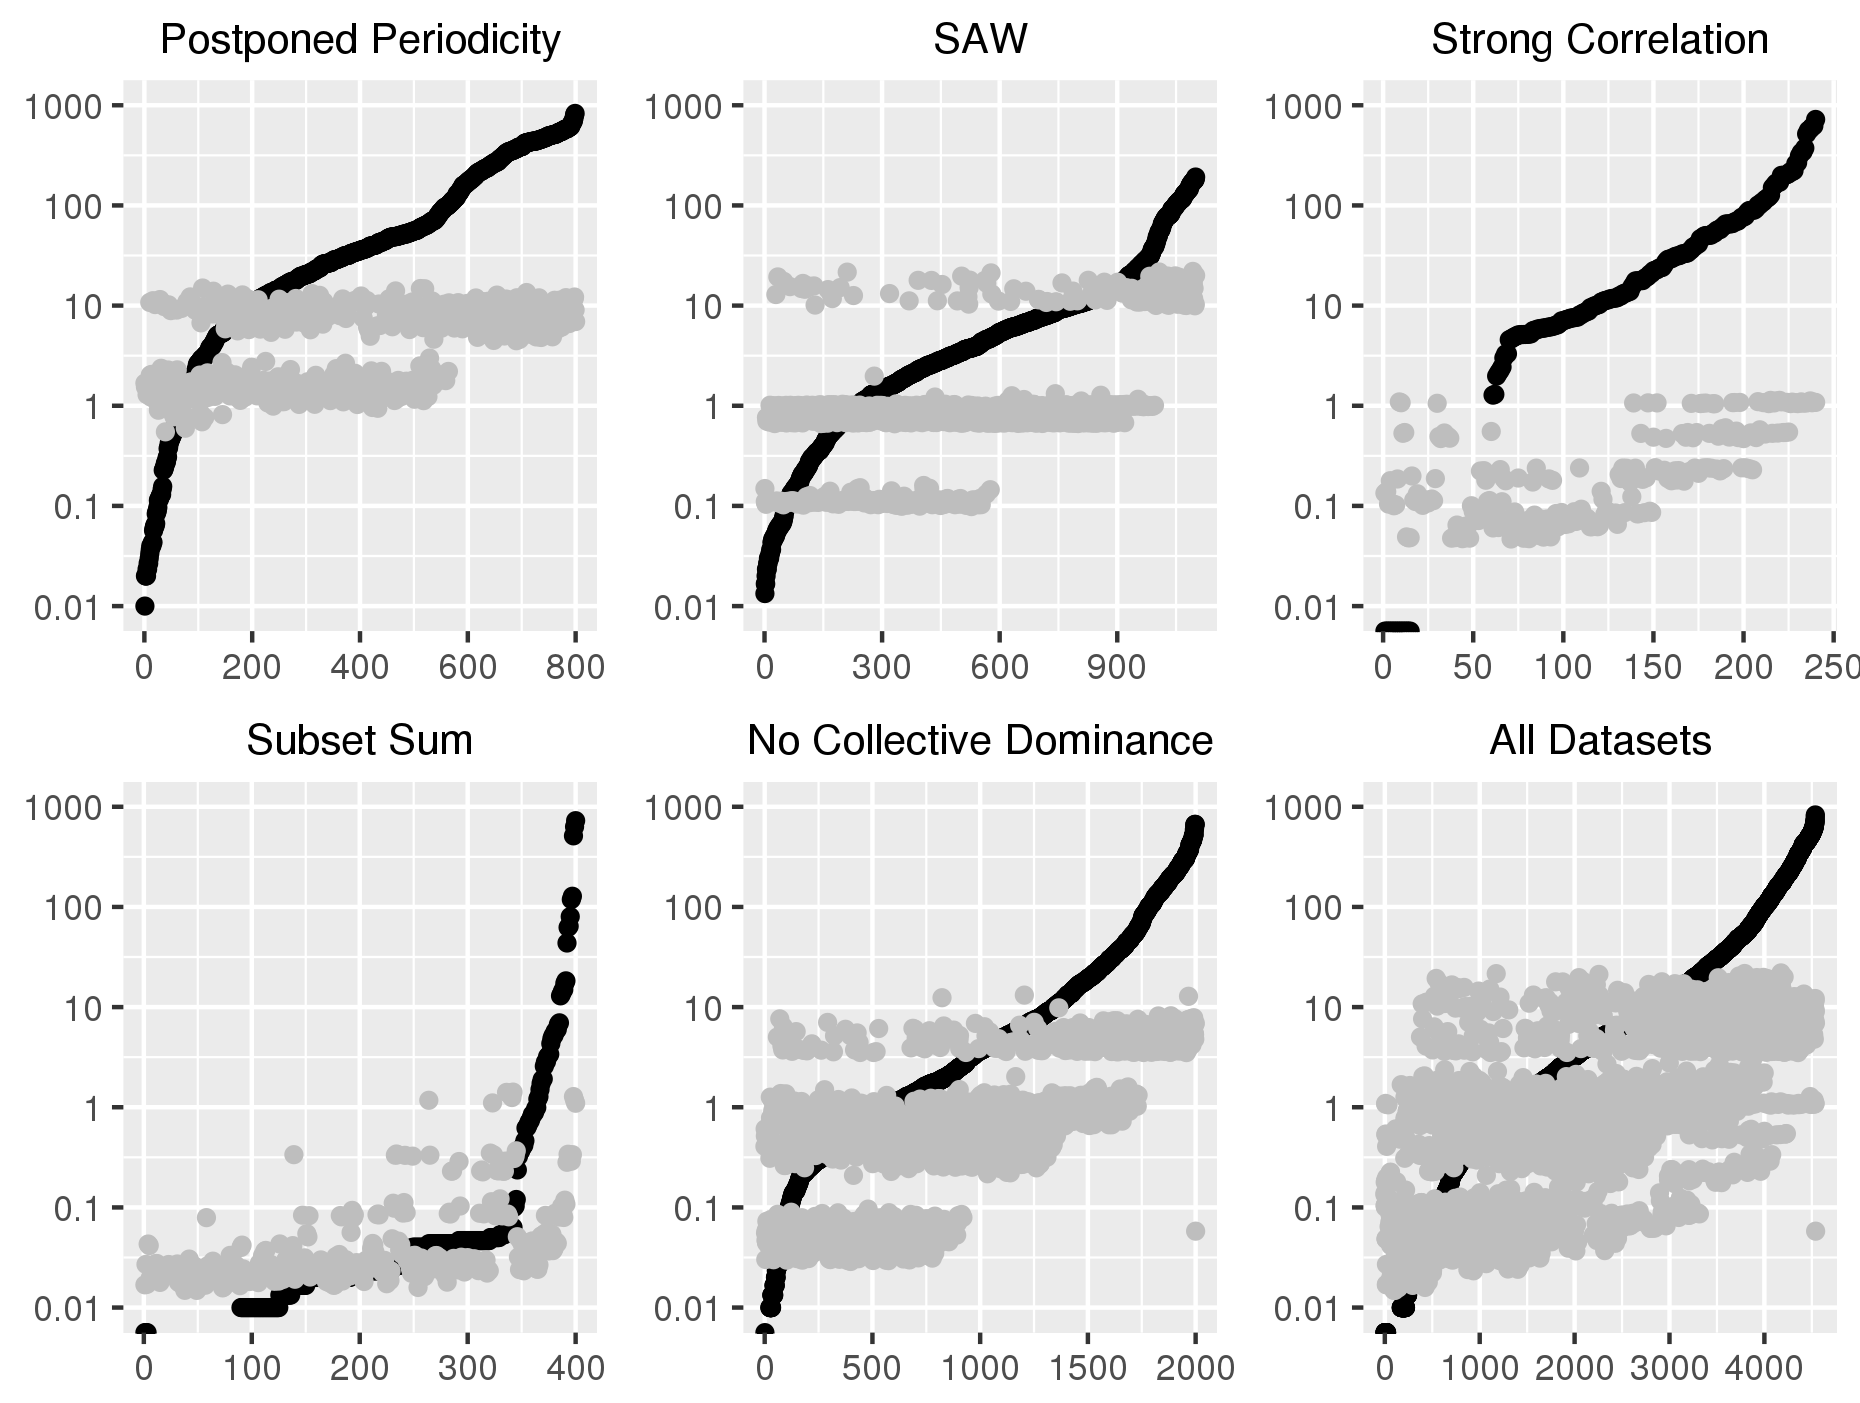
\includegraphics[width=\textwidth]{six_plots.png}
  \caption{The times used by UKP5 and PYAsUKP for each instance of each class. The black dots represent PYAsUKP times. The gray dots represent UKP5 times. The y axis is the time used to solve an UKP instance, in seconds. The x axis is the instance index when the instances are are sorted by the time PYAsUKP took to solve it. Note that the y axis is in logarithmic scale.}
\end{figure}

The computer used on the experiments was an ASUS R552JK-CN159H (Intel Core i7-4700HQ Processor, 6M Cache, 3.40 GHz).
The operating system used was Linux 4.3.3-2 x86\_64.
The instance sets aim to reproduce the ones described in~\cite{pya}, the same tool was used to generate the datasets (PYAsUKP).
The source can be found at \url{https://github.com/henriquebecker91/masters/tree/v0.1}\footnote{
	The UKP5 implementation is at \textbf{codes/cpp/} and two versions of PYAsUKP are at \textbf{codes/ocaml/}.
	The \emph{pyasukp\_site.tgz} is the version used to generate the instances, and was also available at \url{http://download.gna.org/pyasukp/pyasukpsrc.html}. 
	A more stable version was provided by the authors. 
	This version is in \emph{pyasukp\_mail.tgz} and it was used to solve the instances the results presented in Figure~\ref{fig:times}. 
	The \emph{create\_*\_instances.sh} scripts inside \textbf{codes/sh/} were used to generate the instance datasets.
}. 

\section{Conclusion and Final Remarks}

As we can see in figure~\ref{fig:times}, for many instances PYAsUKP is faster than UKP5. However, PYAsUKP can also be one or more orders of magnitude slower than UKP5 on some instances. Our tests have shown when PYAsUKP is faster than UKP5 this is often because of its B\&B phase, that solves some instances almost instantly. When B\&B fails to solve the instance in a short time, PYAsUKP fallbacks to a DP algorithm that seems to be many times slower than UKP5. It's important to note that the asymptotic complexity of both algorithms is pseudo-polynomial (\(O(c\times n)\)), but the difference on the constant factor seems big. Integrating a B\&B phase to UKP5 seems promising, and will be the theme for future works.\vspace{1mm}\\
\textbf{Acknowledgments}
%We are very thankful to Vincent Poirriez for providing us the codes of a stable version of PYAsUKP, and answering our questions about the paper~\cite{pya}. 
We are thankful to the CNPq (Conselho Nacional de Desenvolvimento Cient\'ifico e Tecnol\'ogico) for the financial support.

\bibliographystyle{sbc}
\bibliography{sbc-template}

\end{document}
